\documentclass[tikz]{standalone}
\usetikzlibrary{arrows, positioning}
\tikzset{
  treenode/.style = {align=center, inner sep=1pt, text centered,
    font=\sffamily},
  bst/.style = {treenode, circle, black, font=\sffamily\bfseries, draw=black, text width=2em}
}
\begin{document}
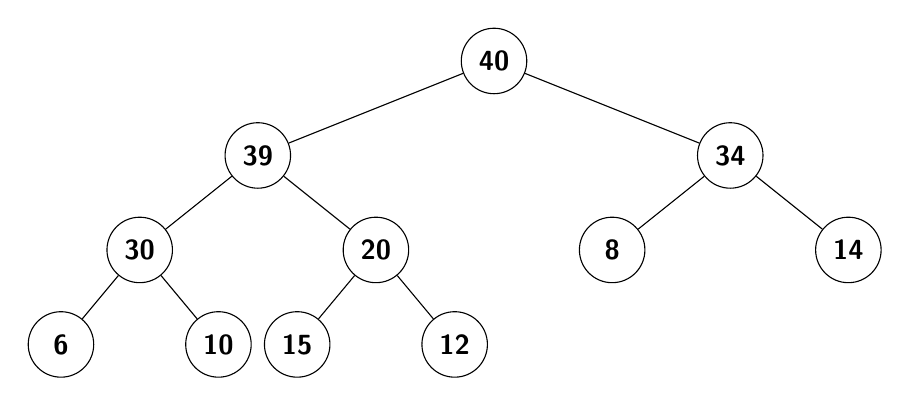
\begin{tikzpicture}[level/.style={sibling distance = 6cm/#1,
  level distance = 1.2cm}]
\node [bst] {40}
    child {node [bst] {39}
        child {node [bst] {30}
            child {node [bst] {6}}
            child {node [bst] {10}}
        }
        child {node [bst] {20}
            child {node [bst] {15}}
            child {node [bst] {12}}
        }
    }
    child { node [bst] {34}
        child{node [bst] {8}}
        child{node [bst] {14}}
    }
;
\end{tikzpicture}
\end{document}
